\documentclass[10pt,a4paper]{article}

\usepackage[linguistics]{forest}
\PassOptionsToPackage{usenames,dvipsnames,svgnames}{xcolor}  
\usepackage{tikz}
\usetikzlibrary{arrows,positioning,automata}
\usepackage{mathtools}
\usepackage{listings}
\usepackage{xcolor}
\usepackage{booktabs} % For prettier tables
\usepackage{multirow} % Required for multirows
\usepackage{siunitx} 
\sisetup{
  round-mode          = places,
  round-precision     = 2,
}
\usepackage{siunitx} % Required for alignment
\sisetup{
  round-mode          = places, % Rounds numbers
  round-precision     = 2, % to 2 places
}
\usepackage{amsmath}
\usepackage{xepersian}
\settextfont{XB Zar}

\begin{document}
	\title{امتحان طراحی الگوریتم}
	\date{1399/مرداد}
	\author{احسان رجبی وحدت}
	\pagenumbering{gobble}
	\maketitle
	\newpage
	\pagenumbering{arabic}
	\paragraph{سوالات نیمسال اول 98-99}
سوالات زوج

	\paragraph{2)} زمان اجرایT(n) به صورت زیر می باشد، پیچدگی زمانی آن کدام است؟
	\begin{flushleft}                           
		$T(n) = 4n + 5nlog(n) + 2$
	\end{flushleft}
	\begin{flushright} 
		1. O(n)\,\,\,\,\, 2. O(n2logn)\,\,\,\,\, \textcolor{blue}{3. O(nlogn)}\,\,\,\,\, 4. O(logn)
	\end{flushright}
	\begin{flushright} 
		\textcolor{blue}{پاسخ:}
	ترتیب مرتبه زمانی از کوچک تر به بزرگ تر:
		$O(1)<O(logn)<O(n)<O(nlogn)<O(n^2)<O(2^n)<O(n^n)<O(n!)$
	\\ در چند جمله ای داده شده جمله $5nlogn$ دارای بالاترین مرتبه زمانی است پس $O(nlogn)$
	\end{flushright}

	\paragraph{4)} پیچیدگی زمانی حاصل ضرب دو ماتریس $n*n$ چیست؟
	\begin{flushright} 
		1. $T(n)\,\,\varepsilon\,\,\theta(n^2)$\,\,\,\,\, \textcolor{blue}{2.$T(n)\,\,\varepsilon\,\,\theta(n^3)$}\,\,\,\,\, 3.$T(n)\,\,\varepsilon\,\,\theta(n^4)$\,\,\,\,\, 4.$T(n)\,\,\varepsilon\,\,\theta(n)$
	\end{flushright}
	\begin{flushright} 
		\textcolor{blue}{پاسخ:}
	تعداد ضرب های حاصل ضرب دو ماتریس $n*n$ برابر می شود با $n*n*n$، پس مرتبه زمانی آن برابر است با $n^3$
	\end{flushright}

	\paragraph{6)} در روش بازگشتی فیبوناچی $Fib(4) + Fib(3)$ چه مقداری را بر می گرداند؟
	\begin{flushright} 
		\textcolor{blue}{1.\,\,5}\,\,\,\,\, 2.\,\,3\,\,\,\,\, 3.\,\,4\,\,\,\,\, 4.\,\,2
	\end{flushright}
	\begin{flushright} 
		\textcolor{blue}{پاسخ:}
		\begin{equation*}
			\begin{split}
				Fib(1)&=1 \\
				Fib(0)&=1 \\
				Fib(2)&=Fib(1)+Fib(0)=2 \\
				Fib(3)&=Fib(2)+Fib(1)=3 \\
				Fib(4)&=Fib(3)+Fib(2)=5 \\
			\end{split} 
		\end{equation*}
	طبق محاسبات فوق جواب مسئله برابر 5 است.
	\end{flushright}

	\paragraph{8)} فرض کنید $a\ge1$ و $b\ge1$ ثابت بوده و $F(n)$ یک تابع بر حسب n باشد $T(n)$ کدام است؟
	\begin{flushright} 
		1.$T(n)=aT(\frac{a}{b})+F(n)$\,\,\,\,\, \textcolor{blue}{2.$T(n)=aT(\frac{n}{b})+F(n)$}\,\,\,\,\,\,\,\,\,\, 3.$T(n)=2T(\frac{a}{b})+F(n)$\,\,\,\,\, 4.$T(n)=2T(\frac{a}{2})+F(b)$
	\end{flushright}
	\begin{flushright} 
		\textcolor{blue}{پاسخ:}
	تابع بازگشتی به صورت $T(n)$ بیان می گردد و باید تابع T بر اساس n بین شود، پس گزینه های 1 و 3 و 4 غلط هستند.
	\end{flushright}

	\paragraph{10)} بدترین حالت زمانی الگوریتم BinsSrch برای جستجوی موفق و ناموفق کدام است؟
	\begin{flushright} 
		1.\,\,$
		T(n) \,\,\varepsilon
		\begin{cases}
			O(logn) & \text{برای جستجوی موفق}\\
			O(logn) & \text{برای جستجوی ناموفق}
		\end{cases}
		$\,\,\,\,\, 2.\,\,$
		T(n) \,\,\varepsilon
		\begin{cases}
		O(logn) & \text{برای جستجوی ناموفق}\\
		\theta(logn) & \text{برای جستجوی موفق}
		\end{cases}
		$\,\,\,\,\, \textcolor{blue}{3.\,\,$
		T(n) \,\,\varepsilon
		\begin{cases}
		O(logn) & \text{برای جستجوی موفق}\\
		\theta(logn) & \text{برای جستجوی ناموفق}
		\end{cases}
		$}\,\,\,\,\, 4.\,\,$
		T(n) \,\,\varepsilon
		\begin{cases}
		O(logn) & \text{برای جستجوی ناموفق}\\
		O(logn) & \text{برای جستجوی موفق}
		\end{cases}
		$
	\end{flushright}
	\begin{flushright} 
		\textcolor{blue}{پاسخ:}
		\begin{table}[]
			\begin{tabular}{ccccr}
				\cline{1-4}
				\multicolumn{1}{|c|}{}              & \multicolumn{1}{c|}{بهترین حالت} & \multicolumn{1}{c|}{میانگین} & \multicolumn{1}{c|}{بدترین حالت} &  \\ \cline{1-4}
				\multicolumn{1}{|c|}{جستجوی موفق}   & \multicolumn{1}{c|}{$\Omega(1)$}         & \multicolumn{1}{c|}{$\theta(logn)$}  & \multicolumn{1}{c|}{$O(logn)$}      &  \\ \cline{1-4}
				\multicolumn{1}{|c|}{جستجوی ناموفق} & \multicolumn{1}{c|}{$\Omega(logn)$}      & \multicolumn{1}{c|}{$\theta(logn)$}  & \multicolumn{1}{c|}{$\theta(logn)$}      &  \\ \cline{1-4}
				\multicolumn{1}{r}{}                & \multicolumn{1}{r}{}             & \multicolumn{1}{r}{}         & \multicolumn{1}{r}{}             & 
			\end{tabular}
		\end{table}
	طبق جدول فوق گزینه 3 پاسخ صحیح می باشد.
	\end{flushright} 

	\paragraph{12)} در ماتریس استراسن ماتریس P چگونه بدست می آید؟
	\begin{flushright} 
		1.$P=(A11 - A22)(B11 + B22)$\,\,\,\,\, \textcolor{blue}{2.$P=(A11 + A22)(B11 + B22)$}\,\,\,\,\, 3.$P=(A11 - A22)(B11 - B22)$\,\,\,\,\, 4.$P=(A11 + A22)(B11 - B22)$
	\end{flushright}
	\begin{flushright} 
		\textcolor{blue}{پاسخ:}
	در ماتریس استراسن:
		\begin{latin}
		$$
			\begin{cases}
				P= & (A_{11}+A_{22})(B_{11}+B_{22}) \\
				Q= & (A_{21}+A_{22})B_{11} \\
				R= &  A_{11}(B_{12}+B_{22}) \\
				S= &  A_{22}(B_{21}+B_{11}) \\
				T= &  (A_{11}+A_{12})B_{22} \\
				U= &  (A_{21}+A_{11})(B_{11}+B_{12}) \\
				V= &  (A_{12}+A_{22})(B_{21}+B_{22})
			\end{cases}
		$$
		\end{latin}
	\end{flushright}

	\paragraph{14)} در ضرب اعداد صحیح بزرگ U و V برابر مقادیر زیر است. مقدار m برابر با چه مقدار می باشد؟
	\begin{flushleft}                           
		$U = X*10m + y$\\
		$V = W*10m + z$
	\end{flushleft}
	\begin{flushright} 
		1.$m=\lfloor\frac{2n}{2}\rfloor$\,\,\,\,\, \textcolor{blue}{2.$m=\lfloor\frac{n}{2}\rfloor$}\,\,\,\,\, 3.$m=\lfloor\frac{2n}{3}\rfloor$\,\,\,\,\, 4.$m=\lfloor\frac{2n}{2}\rfloor$
	\end{flushright}
	\begin{flushright} 
		\textcolor{blue}{پاسخ:}
	اعداد صحیح بزرگ نصف می شوند و اگر n رقم داشته باشند از وسط به دو عدد تبدیل می شوند مثلا U به x و y تبدیل می شود و $m=\lfloor\frac{n}{2}\rfloor$.
	\end{flushright}

	\paragraph{16)} پیچیدگی زمانی الگوریتم پرایم کدام است؟
	\begin{flushright} 
		1.$\theta(n^3)$\,\,\,\,\, \textcolor{blue}{2.$\theta(n^2)$}\,\,\,\,\, 3.$\theta(n)$\,\,\,\,\, 4.$\theta(nm)$
	\end{flushright}
	\begin{flushright} 
		\textcolor{blue}{پاسخ:}
	از آنجا که در الگوریتم پرایم در هر مرحله فاصله هر گره با گره های قبلی مقایسه می شود، پس بدیهی است که از مرتبه $\theta(n^2)$ می باشد که n تعداد رئوس گراف است.
	\end{flushright}

	\paragraph{18)} فرض کنید زمان های ارائه خدمات برای سه کار به صورت زیر می باشد، طبق الگوریتم زمان بندی جواب بهتر کدام است؟
	\begin{flushleft}                           
		$T1 = 12\,\, , \,\, T2 = 7\,\, , \,\, T3 = 10$
	\end{flushleft}
	\begin{flushright} 
		1.$T(n)\,\varepsilon\,\theta(logn)$\,\,\,\,\, \textcolor{blue}{2.$T(n)\,\varepsilon\,\theta(nlogn)$}\,\,\,\,\, 3.$T(n)\,\varepsilon\,O(logn)$\,\,\,\,\, 4.$T(n)\,\varepsilon\,O(nlogn)$
	\end{flushright}
	\begin{flushright} 
		\textcolor{blue}{پاسخ:}
	پیچیدگی الگوریتم بالا برابر است با $T(n)\,\varepsilon\,\theta(nlogn)$.
	\end{flushright}

	\paragraph{20)} در الگوریتم فلوید برای کوتاه ترین مسیر با توجه به گراف زیر مقدار $D_1[2][4]$ چند است؟

	\begin{flushright} 
		1.\,\,5\,\,\,\,\, 2.\,\,4\,\,\,\,\, 3.\,\,3\,\,\,\,\, \textcolor{blue}{4.\,\,2}
	\end{flushright}

	\begin{flushright} 
		\textcolor{blue}{پاسخ:}
		$D_0$ همان ماتریس مجاورت گراف می باشد
		$$
		D_{0} = 
		\begin{bmatrix}
			0 & 1 & \infty & 1 & 5 \\
			9 & 0 & 3 & 2 & \infty \\
			\infty & \infty & 0 & 4 & \infty \\
			\infty & \infty & 2 & 0 & 3 \\
			3 & \infty & \infty & \infty & 0 \\
		\end{bmatrix}
		$$
	برای $D_1$ داریم: ابتدا سطر و ستون 1 را مانند جدول قبل قرار می دهیم
		$$D_1(2,2) , D_1(3,3) , D_1(4,4) \xrightarrow{i=j} \text{برابر با}\,\, 0 
		$$
		$$D_1(2,3) = min(D_0(2,1) + D_0(1,3),D_0(2,3)) = min(9 + \infty,3)=3$$
		$$D_1(2,4) = min(D_0(2,1) + D_0(1,4),D_0(2,4)) = min(9 + 1,2)=2$$
	کوتاه ترین مسیر از گره 2 به گره 4 با گره واسطه 1 برابر است با 2.
	\end{flushright}
	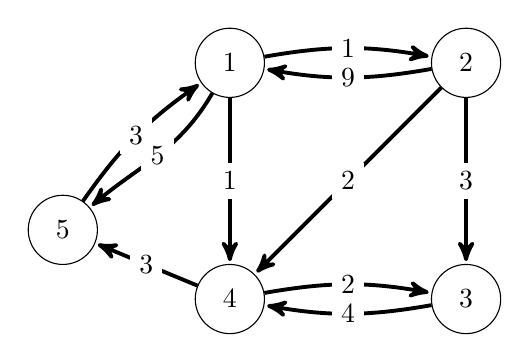
\begin{tikzpicture}[>=stealth',shorten >=1pt,node distance=3cm,on grid,initial/.style    ={}]
		\node[state]          (1)                        {$1$};
		\node[state]          (2) [right =of 1]    {$2$};
		\node[state]          (3) [below =of 2]    {$3$};
		\node[state]          (4) [below =of 1]    {$4$};
		\node[state]          (5) [below left =of 1]    {$5$};
		\tikzset{mystyle/.style={->,double=black}} 
		\tikzset{every node/.style={fill=white}} 
		\path (1)     edge [mystyle]    node   {$1$} (4)
			  (4)     edge [mystyle]    node   {$3$} (5) 
			  (2)     edge [mystyle]    node   {$3$} (3)
			  (2)     edge [mystyle]    node   {$2$} (4);
		\tikzset{mystyle/.style={->,relative=false,in=40,out=240,double=black}}
		\path (1)     edge [mystyle]   node   {$5$} (5); 
		\tikzset{mystyle/.style={->,relative=false,in=215,out=55,double=black}}
		\path (5)     edge [mystyle]   node   {$3$} (1); 

		\tikzset{mystyle/.style={->,relative=false,in=170,out=10,double=black}}
		\path (1)     edge [mystyle]   node   {$1$} (2); 
		\tikzset{mystyle/.style={->,relative=false,in=350,out=190,double=black}}
		\path (2)     edge [mystyle]   node   {$9$} (1);
		
		\tikzset{mystyle/.style={->,relative=false,in=350,out=190,double=black}}
		\path (3)     edge [mystyle]   node   {$4$} (4); 
		\tikzset{mystyle/.style={->,relative=false,in=170,out=10,double=black}}
		\path (4)     edge [mystyle]   node   {$2$} (3);
	\end{tikzpicture}

	\paragraph{22)} در مسئله حاصل جمع زیر مجموعه ها فرض کنید n=5 وW=21 بوده و اعداد داده شده به صورت زیر باشد، تمام زیر مجموعه های Wi های فوق چه مقدار می باشد؟
	\begin{flushleft}
		$W1=5 \,\,\,\, W2=6 \,\,\,\, W3=10 \,\,\,\, W4= 11 \,\,\,\, W5=16$
	\end{flushleft}
	\begin{flushright} 
		1.\,\,19\,\,\,\,\, 2.\,\,20\,\,\,\,\, \textcolor{blue}{3.\,\,21}\,\,\,\,\, 4.\,\,22
	\end{flushright}
	\begin{flushright} 
		\textcolor{blue}{پاسخ:}
	در مسئله حاصل جمع زیر مجموعه ها، می بایست تمام زیر مجموعه هایی از قطعات را بیابیم به طوری که مجموع اوزان آنها به اندازه وزن کوله یعنی 21 باشد.
	\end{flushright}

	\paragraph{24)} پیچیدگی رابطه زیر با روش حدس و استقرا دارای چه مقداری می باشد؟
	\begin{flushleft}
		$T(n)=T(\lfloor\frac{n}{2}\rfloor)+T(\lceil\frac{n}{2}\rceil)+1$
	\end{flushleft}
	\begin{flushright} 
		1.$T(n)\,\varepsilon\,O(nlogn)$\,\,\,\,\, \textcolor{blue}{2.$T(n)\,\varepsilon\,O(n)$}\,\,\,\,\, 3.$T(n)\,\varepsilon\,O(nm)$\,\,\,\,\, 4.$T(n)\,\varepsilon\,O(n^2)$
	\end{flushright}
	\begin{flushright} 
		\textcolor{blue}{پاسخ:}
	با استفاده از قضیه اصلی داریم:
	$$
		2T(\frac{n}{2})+1 \to \begin{cases} &a=2 \\ &b=2 \\ &k=0 \end{cases} \to \begin{cases} & a>b^k \\ & 2>2^0 \end{cases} \to O(n^{\log_b a}) = O(n^{\log_2 2}) = O(n)
		$$
	\end{flushright}

	\paragraph{}
	سوالات تشریحی
	\paragraph{2)} فرض کنید لیستی حاوی عناصر زیر باشد، الگوریتم مرتب سازی سریع را بروی لیست اعمال کنید.
	\begin{flushleft}
		\begin{latin}
			17 \; 20 \; 10 \; 25 \; 11 \; 8 \; 18 \; 23
		\end{latin}
	\end{flushleft}
	\begin{flushright} 
		\textcolor{blue}{پاسخ:}
	ابتدا j در عنصر کوچک تر از 17 متوقف شده و سپس i در عنصر بزرگ تر 17 و پس از آن عناصر تعویض می شوند.
	شماره خانه اول که برابر عدد 17 است معیار قرار می گیرد. j برابر 10 و  i برابر 20 می شود و این دو باهم تعویض میشوند.
		\begin{latin}
			17 \; \textcolor{red}{10} \; \textcolor{red}{20} \; 25 \; 11 \; 8 \; 18 \; 23
		\end{latin}
		j در مرحله بعدی برابر 11 می شود و i برابر عدد 20 و تعویض بعدی بین این دو عدد می باشد.
		\begin{latin}
		17 \; 10 \; \textcolor{red}{11} \; 25 \; \textcolor{red}{20} \; 8 \; 18 \; 23
		\end{latin}
	در مرحله بعدی j برابر 8 و i برابر 25 می شود و دوباره این دو جا به جا می شوند.
		\begin{latin}
		17 \; 10 \; 11 \; \textcolor{red}{8} \; 20 \; \textcolor{red}{25} \; 18 \; 23
		\end{latin}
	اگر j کل آرایه را پیمایش کند و عنصر کوچکتر نباشد محل i با عنصر اول جابجا می شود، پس داریم:
		\begin{latin}
		\textcolor{red}{8} \; 10 \; 11 \; \textcolor{red}{17} \; 20 \; 25 \; 18 \; 23
		\end{latin}
	حال آرایه ما تا عنصر 17 مرتب شده است و حالا عدد 20 معیار قرار میگیرد. پس j برابر با 18 و i برابر با 25 می شود و این دو با هم تعویض می شوند.
		\begin{latin}
		20 \; \textcolor{red}{18} \; \textcolor{red}{25} \; 23
		\end{latin}
	و دوباره عدد 20 با عنصر i جا به جا می شود.
		\begin{latin}
		\textcolor{red}{18} \; \textcolor{red}{20} \; 25 \; 23
		\end{latin}
	حال عدد 25 به عنوان معیار قرار می گیرد و j برابر 23 و i موجود نیست، پس این تعویض نیز انجام می شود و آرایه مرتب می شود.
		\begin{latin}
		\textcolor{red}{23} \; \textcolor{red}{25}
		\end{latin}
	\end{flushright}

	\paragraph{4)} گراف زیر را در نظر بگیرید، درخت پوشای مینیمم گراف بالا را با استفاده از الگوریتم پریم بدست آوردید؟
	\begin{flushright} 
		\textcolor{blue}{پاسخ:}
	در الگوریتم پریم، در هر بار راس جدیدی به مجموعه اضافه می گردد با این شرط که این راس با وزن یال کمتری به مجموعه وصل شود. ابتدا $V_0$ را در نظر می گیریم از مجموعه رئوسی که به آن متصل است راس $V_1$ با کمترین وزن انتخاب می شود، سپس از مجموعه رئوس دیگری که به رئوس $V_0$ و $V_1$ متصلند $V_2$ با کمترین وزن انتخاب می شود راس سوم $V_2$ خواهد بود و به همین ترتیب ...
		\begin{tikzpicture}[>=stealth',shorten >=1pt,node distance=2cm,on grid,initial/.style    ={}]
			  \node[state]          (0) 			     {$ٰV_0$};
			  \node[state]          (1) [below left =of 0]    {$V_1$};
			  \node[state]          (2) [below right =of 0]    {$V_2$};
			  \node[state]          (3) [below =of 1]    {$V_3$};
			  \node[state]          (4) [below =of 2]    {$V_4$};
			  \node[state]          (5) [below right =of 3]    {$V_5$};
			  
			\tikzset{mystyle/.style={-,double=black}} 
			\tikzset{every node/.style={fill=white}} 
			\path (0)     edge [mystyle]    node   {$1$} (1)
				  (1)     edge [mystyle]    node   {$1$} (2) 
				  (3)     edge [mystyle]    node   {$9$} (5);
				
			\tikzset{mystyle/.style={-,relative=false,in=340,out=210,double=black}}
				\path (2)     edge [mystyle]   node   {$3$} (3); 
			\tikzset{mystyle/.style={-,relative=fa;se,in=170,out=340,double=black}}
				\path (1)     edge [mystyle]   node   {$5$} (4);

		\end{tikzpicture}
	\end{flushright}

	\newpage
	\paragraph{سوالات نیمسال اول 93-94}
	سوالات فرد

	\paragraph{1)} فرض کنید قطعه برنامه p1 با زمان اجرای T1(n) به موازات قطعه برنامه p2 با زمان اجرای T2(n) اجرا می شود. اگر $T1(n)=O(n^2)$ و $T2(n)=O(nlogn)$ باشد. مقدارT1(n)+T2(n) کدام است؟
	\begin{flushright} 
		1.$O(n^2logn)$\,\,\,\,\, \textcolor{blue}{2.$O(n^2)$}\,\,\,\,\, 3.$O(nlogn)$\,\,\,\,\, 4.$O(n^3logn)$
	\end{flushright}
	\begin{flushright} 
		\textcolor{blue}{پاسخ:}
ترتیب مرتبه زمانی از کوچک تر به بزرگ تر: \\
			$O(1)<O(logn)<O(n)<O(nlogn)<O(n^2)<O(2^n)<O(n^n)<O(n!)$
	\\به دلیل بزرگ تر بودن مرتبه زمانی $T1(n)$ نسبت به $T2(n)$ پس مرتبه زمانی جمع دو قطعه برنامه برابر $O(n^2)$ می باشد.
	\end{flushright}

	\paragraph{3)}تابع پیچیدگی زمانی برای تابع بازگشتی زیر چیست؟

	\begin{flushleft}
		\begin{latin}
			int F(int n, int m)\{\\
			\hspace{1cm}if(n==1) return n;\\
			\hspace{1cm}else\\
			\hspace{2cm}return F(n-1,m-1)*F(n-2,m)\\
			\}
		\end{latin}
	\end{flushleft}
	\begin{flushright} 
		1.$T(n,m)=T(n-1,m-1)*T(n-2,m)+n$\,\,\,\,\, 2.$T(n)=T(n-1)*T(n-2)+n$\,\,\,\,\, 3.$T(n,m)=T(n-1,m-1)*T(n-2,m)+1$\,\,\,\,\, \textcolor{blue}{4.$T(n,m)=T(n-1)*T(n-2)+1$}
	\end{flushright}
	\begin{flushright} 
		\textcolor{blue}{پاسخ:}
		اگرT(n,m) را به عنوان $F(n-1,m-1)*F(n-2,m)$ در نظر بگیریم با توجه به شرط else تابع، $T(n,m) =T(n-1,m-1)*T(n-2,m) $ می باشد اما با توجه به اینکه m در زمان اجرا تاثیری ندارد و همچنین خود شرط if مرتبه زمانی 1 دارد پس $T(n,m)=T(n-1)*T(n-2)+1$ می باشد.
	\end{flushright}

	\paragraph{5)} خروجی تابع بازگشتی f به ازای درخت دودویی زیر چیست؟

	\begin{minipage}{.40\linewidth}
		\begin{flushright}

			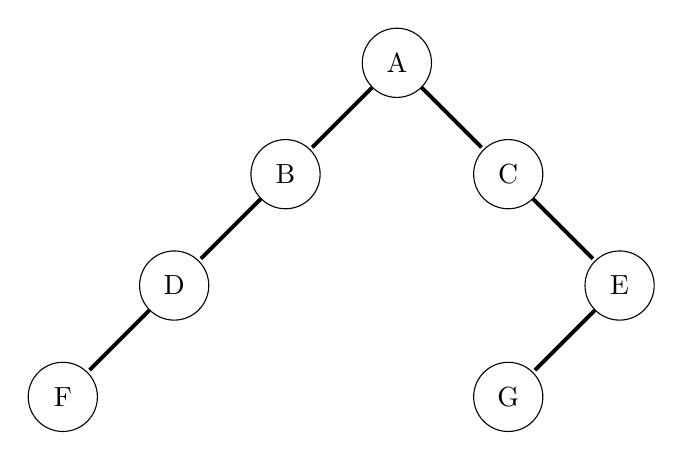
\begin{tikzpicture}[>=stealth',shorten >=1pt,node distance=2cm,on grid,initial/.style    ={}]
				  \node[state]          (A) 			     {A};
				  \node[state]          (B) [below left =of A]    {B};
				  \node[state]          (C) [below right =of A]    {C};
				  \node[state]          (D) [below left =of B]    {D};
				  \node[state]          (E) [below right =of C]    {E};
				  \node[state]          (F) [below left =of D]    {F};
				  \node[state]          (G) [below left =of E]    {G};
				  
				\tikzset{mystyle/.style={-,double=black}} 
				\path (A)     edge [mystyle]    node   {} (B)
					  (B)     edge [mystyle]    node   {} (D) 
					  (A)     edge [mystyle]    node   {} (C)
					  (C)     edge [mystyle]    node   {} (E)
					  (E)     edge [mystyle]    node   {} (G)
					  (D)     edge [mystyle]    node   {} (F);
			\end{tikzpicture}

		\end{flushright}
	\end{minipage}
	 \hfill
	\begin{minipage}{.55\linewidth}
		\begin{flushleft}
		  \begin{latin}
			int f(Node * tree)\{\\
			\hspace{1cm}if(tree==NULL) return 0;\\
			\hspace{1cm}else\{\\
			\hspace{2cm}int i = f(tree -> left);\\
			\hspace{2cm}int j = f(tree -> right);\\
			\hspace{2cm}if (i>j) return 1+i;\\
			\hspace{2cm}else return 1+j;\\
			\hspace{1cm}\}\\
			\}
		 \end{latin}
		\end{flushleft} 
	\end{minipage}
	\begin{flushright} 
		1. 2\,\,\,\,\, 2. 3\,\,\,\,\, \textcolor{blue}{3. 4}\,\,\,\,\, 4. 7
	\end{flushright}
	\begin{flushright} 
		\textcolor{blue}{پاسخ:}
		خروجی تابع f برابر 4 می باشد.
	\end{flushright}

	\paragraph{7)} برای جستجوی عنصر x=40 به روش جستجوی دودویی در آرایه زیر چند مقایسه نیاز است؟
	\begin{flushleft} 
		\begin{latin}
			11 , 12 , 18 , 20 , 21 , 23 , 27 , 40 , 75 , 80 , 85 
		\end{latin}
	\end{flushleft}
	\begin{flushright} 
		1. 2\,\,\,\,\, 2. 3\,\,\,\,\, \textcolor{blue}{3. 4}\,\,\,\,\, 4. 5
	\end{flushright}
	\begin{flushright} 
		\textcolor{blue}{پاسخ:}\\
		مقایسه 1: x با عنصر خانه $[\frac{1+11}{2}]=6$ چون 40>23 پس مقایسه بعدی در نیمه بالایی آرایه است. \\
		مقایسه 2: x با عنصر خانه $[\frac{7+11}{2}]=9$ چون 75>40 پس مقایسه بعدی در نیمه پایینی آرایه است. \\
		مقایسه 3: x با عنصر خانه $[\frac{7+8}{2}]=7$ چون 40>27 پس مقایسه بعدی در نیمه بالایی آرایه است. \\ 
		مقایسه 4: x با عنصر خانه $[\frac{8+8}{2}]=8$ در این مقایسه 40=40 یافت شد.
	\end{flushright}:

	\paragraph{9)} آرایه زیر را در نظر بگیرید. اگر عنصر اول آرایه یعنی عدد 9 به عنوان لولا اختیار شود. کدام گزینه های زیر می تواند خروجی مرحله اول الگوریتم مرتب سازی سریع باشد؟
	\begin{flushleft} 
		\begin{latin}
			9 , 10 , 8 , 7 , 6 , 15 , 3
		\end{latin}
	\end{flushleft}
	\begin{flushright} 
		1.$6-7-8-9-3-15-10$\,\,\,\,\, 2.$7-8-9-10-3-6-15$\,\,\,\,\, 3.$7-8-9-3-6-10-15$\,\,\,\,\, \textcolor{blue}{4.$3-8-7-6-9-15-10$}
	\end{flushright}
	\begin{flushright} 
		\textcolor{blue}{پاسخ:}
		عنصر آخر که برابر 3 هست می شود معیار ما برای مقایسه، خانه ابتدایی که 9 است برابر i  می شود و چون از 3 بزرگ تر است پس j با پیمایش آرایه باید دنبال عددی کمتر از 3 باشد. و چون یافت نمی شود، پس 9 با 3 جا به جا می شود و به خانه اول می آید. در گزینه ها فقط گزینه 4 است که خانه اول آرایه 3 می باشد. پس با حذف سایر گزینه ها به این جواب میرسیم.
	\end{flushright}

	\paragraph{11)} در صورت استفاده از روش تقسیم و حل، مینیمم و ماکزیمم اعداد ذخیره شده در آرایه یک بعدی با n خانه، با چند مقایسه بین اعداد ذخیره شده در این خانه ها بدست خواهد آمد؟
	\begin{flushright} 
		1.$3\frac{n}{2}$\,\,\,\,\, 2.$\frac{n}{2}$\,\,\,\,\, \textcolor{blue}{3.$3\frac{n}{2}-2$}\,\,\,\,\, 4.$\frac{n+1}{2}$
	\end{flushright}
	\begin{flushright} 
		\textcolor{blue}{پاسخ:}
		\\ برای n فرد $T(n) = 3\frac{n}{2}-\frac{3}{2}$ \\
		برای n زوج $T(n) = 3\frac{n}{2}-2$
	\end{flushright}

	\paragraph{13)} کدام یال از گراف زیر توسط الگوریتم پریم در مرحله سوم انتخاب میشود؟ شروع از راس V0

	\begin{tikzpicture}[>=stealth',shorten >=1pt,node distance=2cm,on grid,initial/.style    ={}]
		  \node[state]          (0) 			     {$ٰV_0$};
		  \node[state]          (1) [below left =of 0]    {$V_1$};
		  \node[state]          (2) [below right =of 0]    {$V_2$};
		  \node[state]          (3) [below =of 1]    {$V_3$};
		  \node[state]          (4) [below =of 2]    {$V_4$};
		  \node[state]          (5) [below right =of 3]    {$V_5$};
		  
		\tikzset{mystyle/.style={-,double=black}} 
		\tikzset{every node/.style={fill=white}} 
		\path (0)     edge [mystyle]    node   {$6$} (1)
			  (0)     edge [mystyle]    node   {$7$} (2)
			  (1)     edge [mystyle]    node   {$4$} (2) 
			  (1)     edge [mystyle]    node   {$5$} (3)
			  (2)     edge [mystyle]    node   {$6$} (4)
			  (3)     edge [mystyle]    node   {$5$} (4)
			  (4)     edge [mystyle]    node   {$2$} (5)
			  (3)     edge [mystyle]    node   {$1$} (5);
				
		\tikzset{mystyle/.style={-,relative=false,in=340,out=210,double=black}}
			\path (2)     edge [mystyle]   node   {$8$} (3); 
		\tikzset{mystyle/.style={-,relative=fa;se,in=170,out=340,double=black}}
			\path (1)     edge [mystyle]   node   {$7$} (4);
	\end{tikzpicture}
	\begin{flushright} 
		1. V4V5\,\,\,\,\, \textcolor{blue}{2. V1V3}\,\,\,\,\, 3. V1V2\,\,\,\,\, 4. V2V4
	\end{flushright}
	\begin{flushright} 
		\textcolor{blue}{پاسخ:}
		\\ مرحله اول: رئوس مجاور $ٰV_0$ برابر {$V_2$ , $V_1$} می باشد، چون 6 کوچک تر از 7 هست پس یال $e_{01}$ انتخاب می شود. \\
		مرحله دوم: حال رئوس مجاور برابر {$V_2$, $V_3$, $V_4$} می باشد، که کوچک ترین یال برابر 4 هست پس یال $e_{12}$ انتخاب می شود. \\
		مرجله سوم: در این مرحله رئوس مجاور برابر {$V_3$, $V_4$} می باشد، که کوچک ترین یال برابر 5 هست پس یال $e_{13}$ انتخاب می شود.
	\end{flushright}

	\paragraph{15)}  اگر رشته abcabbaccaabdffe را به روش کدینگ هافمن کد نماییم. طول کد چند بیت خواهد شد؟
	\begin{flushright}
		1. 34\,\,\,\,\, 2. 35\,\,\,\,\, 3. 36\,\,\,\,\, \textcolor{blue}{4. 38}
	\end{flushright}
	\begin{flushright} 
		\textcolor{blue}{پاسخ:}
		\begin{flushleft}
			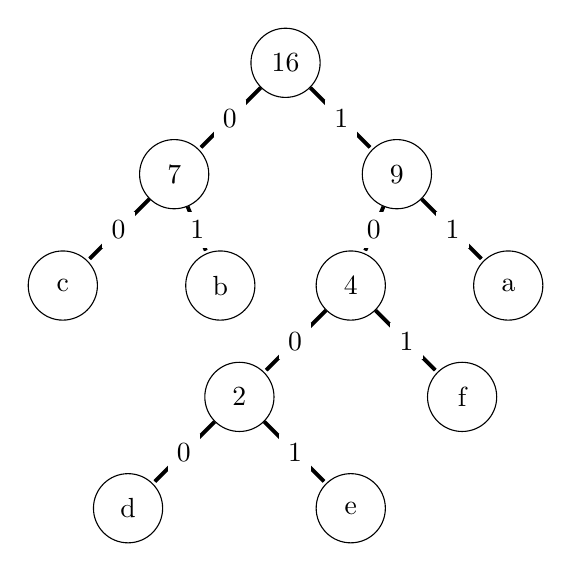
\begin{tikzpicture}[>=stealth',shorten >=1pt,node distance=2cm,on grid,initial/.style    ={}]
				  \node[state]          (16) 			     {$16$};
				  \node[state]          (7) [below left =of 16]    {$7$};
				  \node[state]          (9) [below right =of 16]    {$9$};
				  \node[state]          (a) [below right of= 9]			     {a};
				  \node[state]          (4) [left =of a]    {$4$};
				  \node[state]          (2) [below left =of 4]    {$2$};
				  \node[state]          (c) [below left of= 7]			     {c};
				  \node[state]          (b) [right =of c]    {b};
				  \node[state]          (d) [below left of= 2]			     {d};
				  \node[state]          (e) [below right of= 2]			     {e};
				  \node[state]          (f) [below right of= 4]			     {f};
				  
				  
				\tikzset{mystyle/.style={-,double=black}} 
				\tikzset{every node/.style={fill=white}}
				\path (16)     edge [mystyle]    node   {$0$} (7)
					  (16)     edge [mystyle]    node   {$1$} (9)
					  (7)     edge [mystyle]    node   {$0$} (c) 
					  (7)     edge [mystyle]    node   {$1$} (b)
					  (9)     edge [mystyle]    node   {$0$} (4)
					  (9)     edge [mystyle]    node   {$1$} (a)
					  (4)     edge [mystyle]    node   {$0$} (2)
					  (4)     edge [mystyle]    node   {$1$} (f)
					  (2)     edge [mystyle]    node   {$0$} (d)
					  (2)     edge [mystyle]    node   {$1$} (e);
			\end{tikzpicture}
		\end{flushleft}
		تعداد کل بیت های مورد نیاز برابر با :
			$$
			5*2+4*2+3*2+1*5+2*3+1*4 = 10+8+6+4+6+4 = 38
			$$
	\end{flushright}

	\paragraph{17)} ماتریس های $A13*5$ , $B5*89$ و $D3*34$ را در نظر بگیرید. حداقل تعداد ضرب مورد نیاز برای محاسبه $M=A*B*C*D$ کدام است؟
	\begin{flushright} 
		1. 4055\,\,\,\,\, 2. 54201\,\,\,\,\, 3. 3425\,\,\,\,\, \textcolor{blue}{4. 2856}
	\end{flushright}
	\begin{flushright} 
		\textcolor{blue}{پاسخ:}
		\begin{align}
			A_{13*5}B_{5*89}C_{89*3}D_{3*34} &= A_{13*5}(BC)_{5*3}D_{3*34} = (A(BC))_{13*3}D_{3*34} \notag\\
			&= ((A(BC))D)_{13*34} \notag \\
			5*89*3 + 13*5*3 + 13*3*14 &= 2856 \notag
		\end{align}
	\end{flushright}

	\paragraph{19)} با n عنصر مختلف، چند درخت جستجوی دودویی متفاوت با ارتفاع n-1 وجود دارد?
	\begin{flushright} 
		\textcolor{blue}{1.$2^{n-1}$}\,\,\,\,\, 2.$n!$\,\,\,\,\, 3.$2^n$\,\,\,\,\, 4. 1
	\end{flushright}
	\begin{flushright} 
		\textcolor{blue}{پاسخ:} \\
		با n گره عمق n-1 یعی در هر سطح فقط یک گره. با n گره میتوان ابتدا یک گره را به عنوان ریشه در نظر گرفت سپس در عمق 1 برای گره بعدی دو حالت داریم یا فرزند راست یا فرزند چپ، در عمق 2 هم برای هر گره دو حالت داریم و ... \\
		لذا تعداد کل حالات برابر است با: \\
		$(2*2*...*2) = 2^{n-1}$
		\\ چون گره ریشه یک حالت دارد لذا n-1 گره دیگر می توانند دو حالت داشته باشند. 
	\end{flushright}

	\paragraph{21)} فرض کنید دو وزیر در نقاط (i,j) و (k,l) روی یک صفحه شطرنج n*n قرار گرفته اند. کدام یک از گزینه های زیر هم قطر بودن آن ها را تعیین می کند؟
	\begin{flushright} 
		1. (i==k) OR (j==l)\,\,\,\,\, 2. (i-k) OR (j-l)\,\,\,\,\,\\ \textcolor{blue}{3. (i-j==k-l) OR (i+j==k+l)}\,\,\,\,\, 4. (i-k==j-l) OR (i-k==l+n-j)
	\end{flushright}
	\begin{flushright} 
		\textcolor{blue}{پاسخ:}
		با مثال حل میکنیم: \\
		$(i,j)->(k,l)$ \\
		$(2,5)->(4,3)$ \\
		$(2,5)->(5,8)$ \\
		\begin{latin} if (|i-k|=|j-l|) then \end{latin}
	\end{flushright}

	\paragraph{23)} در حل مساله فروشنده دوره گرد به روش انشعاب و تحدید، درخت فضای حالت بدست آمده در مرحله سوم به شکل زیر است. در مرحله بعد کدام گره از درخت باید توسعه یابد؟
	\begin{flushleft}
		\begin{tikzpicture}[>=stealth',shorten >=1pt,node distance=2cm,on grid,initial/.style    ={}]
			  \node[state]          (20) 			     {$20$};
			  \node[state]          (32) [below left =of 20]    {$32_{(C)}$};
			  \node[state]          (29) [below right =of 20]    {$29_{(D)}$};
			  \node[state]          (24) [left =of 32]    {$24$};
			  \node[state]          (42) [right =of 29]    {$42$};
			  \node[state]          (31) [below of= 24]			     {$ٰ31_{(A)}$};
			  \node[state]          (25) [left =of 31]    {$24$};
			  \node[state]          (41) [right of= 31]			     {$ٰ41_{(B)}$};
			  \node[state]          (37) [below left of= 25]			     {$ٰ37$};
			  \node[state]          (33) [below right of= 25]			     {$ٰ32$};
			  
			\tikzset{mystyle/.style={-,double=black}} 
			\path (20)     edge [mystyle]    node   {} (24)
				  (20)     edge [mystyle]    node   {} (32)
				  (20)     edge [mystyle]    node   {} (29) 
				  (20)     edge [mystyle]    node   {} (42)
				  (24)     edge [mystyle]    node   {} (25)
				  (24)     edge [mystyle]    node   {} (31)
				  (24)     edge [mystyle]    node   {} (41)
				  (25)     edge [mystyle]    node   {} (37)
				  (25)     edge [mystyle]    node   {} (33);
		\end{tikzpicture}
	\end{flushleft}
	\begin{flushright} 
		1. A\,\,\,\,\, 2. B\,\,\,\,\, 3. C\,\,\,\,\, \textcolor{blue}{4. D}
	\end{flushright}
	\begin{flushright} 
		\textcolor{blue}{پاسخ:}
		 در روش انشعاب و تحدید یکی از روش های جستجو، جستجوی سطحی است. در ردیف دوم بعد از عدد 24 باید سراغ کمترین اندازه گره برویم که 29 است و نقطه D می شود.
	\end{flushright}

	\paragraph{25)} کدام یک از گزینه های زیر در مورد مسائل کلاس NP صحیح است؟
	\begin{flushright} 
		\textcolor{blue}{1. NP مجموعه تمامی مسائل تصمیم گیری است که توسط الگوریتم های غیر قطعی با زمان چد جمله ای قابل حل است.}\\
	2. همه مسائل NP الگوریتمی کارا با زمان چند جمله ای دارند.\\
	3. طراحی یک الگوریتم با زمان چند جمله ای برای مسائل NP غیر ممکن است.\\
	4. مسائلی که رام نشدنی بودن آنها اثبات شده است در کلاس NP قرار می گیرند.
	\end{flushright}
	\begin{flushright} 
		\textcolor{blue}{پاسخ:} \\
		گزینه 4 غلط می باشد زیرا مسائلی که رام نشدنی بودن آنها اثبات شده است در کلاس NP قرار نمی گیرند. \\
		گزینه 3 غلط می باشد زیرا الگوریتم های زمان چند جمله ای در کلاس NP قرار می گیرند. \\
		گزینه 2 غلط می باشد زیرا لزوما همه مسائل NP الگوریتم با زمان چند جمله ای، الگوریتم کارایی ندارند.
	\end{flushright}

	\newpage
	\paragraph{}
	سوالات تشریحی
	\paragraph{1)} الف) الگوریتم کروسکال را برای پیدا کردن درخت پوشای کمینه گراف زیر بکار برده، مرحله به مرحله عملیات را نشان دهید.\\
	ب) پیچیدگی زمانی این الگوریتم را تحلیل نمایید.
	\begin{flushleft}
		\begin{tikzpicture}[>=stealth',shorten >=1pt,node distance=2cm,on grid,initial/.style    ={}]
			  \node[state]          (1) 			     {$1$};
			  \node[state]          (2) [right =of 1]    {$2$};
			  \node[state]          (4) [below =of 1]    {$4$};
			  \node[state]          (5) [below right =of 2]    {$5$};
			  \node[state]          (3) [right =of 5]    {$3$};
			  \node[state]          (6) [below left of= 5]			     {$ٰ6$};

			  
			\tikzset{mystyle/.style={-,double=black}} 
			\tikzset{every node/.style={fill=white}} 
			\path (1)     edge [mystyle]    node   {$10$} (2)
				  (1)     edge [mystyle]    node   {$30$} (4)
				  (1)     edge [mystyle]    node   {$45$} (5) 
				  (2)     edge [mystyle]    node   {$25$} (6)
				  (2)     edge [mystyle]    node   {$40$} (5)
				  (2)     edge [mystyle]    node   {$50$} (3)
				  (3)     edge [mystyle]    node   {$35$} (5)
				  (3)     edge [mystyle]    node   {$15$} (6)
				  (4)     edge [mystyle]    node   {$20$} (6)
				  (5)     edge [mystyle]    node   {$55$} (6);
		\end{tikzpicture}
	\end{flushleft}
	\begin{flushright} 
		\textcolor{blue}{پاسخ:}
		در الگوریتم کروسکال یال ها را به ترتیب صعودی نسبت به وزن هایشان مرتبی می کنیم سپس یال ها را از کم انتخاب میکنیم و شرط درست نشدن دور را نیز باید رعایت کنیم. \\
		\begin{latin}
			\begin{center}
	 	 		\begin{tabular}{ l | c | r }
					i <-> & j & W \\ \hline
					1 & 2 & 10 \\ \hline
					3 & 6 & 15 \\ \hline
					4 & 6 & 20 \\ \hline
					2 & 6 & 25 \\ \hline
					1 & 4 & 30 \\ \hline
					3 & 5 & 35 \\ \hline
					2 & 5 & 40 \\ \hline
					1 & 5 & 45 \\ \hline
					2 & 3 & 50 \\ \hline
					5 & 6 & 55 \\ 
	 			 \end{tabular}
			\end{center}
		\end{latin}
		
		\begin{flushleft}
			\begin{tikzpicture}[>=stealth',shorten >=1pt,node distance=2cm,on grid,initial/.style    ={}]
				  \node[state]          (1) 			     {$1$};
				  \node[state]          (2) [right =of 1]    {$2$};
				  \node[state]          (4) [below =of 1]    {$4$};
				  \node[state]          (5) [below right =of 2]    {$5$};
				  \node[state]          (3) [right =of 5]    {$3$};
				  \node[state]          (6) [below left of= 5]			     {$ٰ6$};

				  
				\tikzset{mystyle/.style={-,double=black}} 
				\tikzset{every node/.style={fill=white}} 
				\path (1)     edge [mystyle]    node   {$10$} (2)
					  (2)     edge [mystyle]    node   {$25$} (6)
					  (3)     edge [mystyle]    node   {$35$} (5)
					  (3)     edge [mystyle]    node   {$15$} (6)
					  (4)     edge [mystyle]    node   {$20$} (6);
			\end{tikzpicture}
		\end{flushleft}
		پیچیدگی الگوریتم کروسکال برابر است با
		 $\theta(n^2\log{n})$
	\end{flushright}

	\paragraph{3)} فرض کنید سه کلید a1<a2<a3 موجود باشند. اگر احتمال مساوی بودن کلید مورد جستجو با a1=0.7 , a2=0.2 و a3=0.1 باشد. درخت جستجوی دودویی و میانگین زمان جستجوی بهینه را به روش برنامه نویسی پویا بدست آرید؟ عملیات را مرحله به مرلحه نشان دهید.
	\begin{flushright} 
		\textcolor{blue}{پاسخ:}
		$$
		\begin{bmatrix}
			0 & 0.7 & 1.1 & 1.4  \\
			  & 0   & 0.2 & 0.4  \\
			  &     & 0 & 0.1    \\
			  &     &   & 0      \\
		\end{bmatrix}
		$$
	\end{flushright}

	\paragraph{5)} با استفاده از روش انشعاب و تحدید برای مسئله کوله پشتی صفر و یک، سود ماکزیمم قابل حصول از نمونه را پیدا کنید. عملیات را مرحله به مرحله نمایش دهید.\\
	n=5 \; w=22
	\begin{latin}
		\begin{center}
	 	 \begin{tabular}{ l | c | r }
			i & Pi & Wi \\ \hline
			1 & 30\$ & 6 \\ \hline
			2 & 18\$ & 9 \\ \hline
			3 & 3\$ & 3 \\ \hline
			4 & 35\$ & 7 \\ \hline
			5 & 27\$ & 3 \\ 
	 	 \end{tabular}
		\end{center}
	\end{latin}
	\begin{flushright} 
		\textcolor{blue}{پاسخ:}
		یافتن $\frac{P_i}{W_i}$ :
		\begin{latin}
			\begin{center}
	 	 		\begin{tabular}{ l | c | r }
					$\frac{P_i}{W_i}$ & Pi & Wi \\ \hline
					5 & 30\$ & 6 \\ \hline
					3 & 18\$ & 9 \\ \hline
					1 & 3\$ & 3 \\ \hline
					5 & 35\$ & 7 \\ \hline
					9 & 27\$ & 3 \\ 
	 			 \end{tabular}
			\end{center}
		\end{latin}
	\begin{flushleft}
		\begin{tikzpicture}[>=stealth',shorten >=1pt,node distance=2cm,on grid,initial/.style    ={}]
			  \node[state]          (00) 			     {$0, 0, 104$};
			  \node[state]          (11) [below left =of 00]    {$3, 27, 104$};
			  \node[state]          (12) [below right =of 00]    {$0, 0, 83$};
			  \node[state]          (21) [below left =of 11]    {$9, 57, 104$};
			  \node[state]          (22) [below right =of 11]    {$3, 27, 83$};
			  \node[state]          (31) [below left of= 21]			     {$ٰ16, 92, 104$};
			  \node[state]          (32) [below right of= 21]			     {$ٰ9, 57, 78$};
			  \node[state]          (41) [below left of= 31]			     {$ٰ25 > 22$};
			  \node[state]          (42) [below right of= 31]			     {$ٰ16, 92, 95$};
			  \node[state]          (51) [below left of= 42]			     {$ٰ19, 95, 95$};
			  \node[state]          (52) [below right of= 42]			     {$ٰ16, 92, 92$};
			  
			\tikzset{mystyle/.style={-,double=black}} 
			 
			\path (00)     edge [mystyle]    node   {} (11)
				  (00)     edge [mystyle]    node   {} (12)
				  (11)     edge [mystyle]    node   {} (21) 
				  (11)     edge [mystyle]    node   {} (22)
				  (21)     edge [mystyle]    node   {} (31)
				  (21)     edge [mystyle]    node   {} (32)
				  (31)     edge [mystyle]    node   {} (41)
				  (31)     edge [mystyle]    node   {} (42)
				  (42)     edge [mystyle]    node   {} (51)
				  (42)     edge [mystyle]    node   {} (52);
		\end{tikzpicture}
	\end{flushleft}
	سود ماکزیمم برابر میشه با 95.
	\end{flushright}

\end{document}